\documentclass[a4paper]{article}

%%%%%%%%%%%%%%%%%%%%%%%%%%%%%%%%%%%%%%%%%%%%%%%%%%%%%%%%%%%%%%%%%%%%%%%%%%%%
% Some common includes. Add additional includes you need.
%%%%%%%%%%%%%%%%%%%%%%%%%%%%%%%%%%%%%%%%%%%%%%%%%%%%%%%%%%%%%%%%%%%%%%%%%%%%
\RequirePackage{ngerman}
\RequirePackage[utf8]{inputenc}
\RequirePackage[T1]{fontenc}
\RequirePackage[margin=30mm,bottom=40mm]{geometry}
\RequirePackage{graphicx}
\RequirePackage{amsmath,amsfonts,amssymb,amsthm}
\RequirePackage{listingsutf8}
\RequirePackage{textcomp}
\RequirePackage{soul}
\RequirePackage{hyperref}
\RequirePackage{tikz}

\renewcommand{\baselinestretch}{1.15} % Line spacing

\usetikzlibrary{arrows.meta}

%%%%%%%%%%%%%%%%%%%%%%%%%%%%%%%%%%%%%%%%%%%%%%%%%%%%%%%%%%%%%%%%%%%%%%%%%%%%
% Defines for mathematical notation. Add additional defines as needed.
%%%%%%%%%%%%%%%%%%%%%%%%%%%%%%%%%%%%%%%%%%%%%%%%%%%%%%%%%%%%%%%%%%%%%%%%%%%%
\def\O{\mathcal{O}}
\def\sort{\mathrm{sort}}
\def\scan{\mathrm{scan}}
\def\dist{\mathrm{dist}}





\newtheorem{theorem}{Satz}


\theoremstyle{definition}
\newtheorem{definition}{Definition}

\theoremstyle{remark}
\newtheorem*{remark}{Bemerkung}

\def\proofname{Beweis}


\usepackage{listings}
\lstset{%
  showstringspaces=false,
  mathescape=true,
  inputencoding=utf8,
  numbers=left,
  xleftmargin=\parindent,
  basicstyle=\footnotesize\ttfamily,
  keywordstyle=\bfseries\color{green!40!black},
  commentstyle=\normalfont\itshape\color{black!60},
  identifierstyle=\color{blue},
  stringstyle=\color{violet},
  tabsize=2%
}


\begin{document}
	\begin{titlepage}
	
	\begin{center}

		\huge \textbf{\textsf{
		\\Arithmetisches Kodieren}} \\
		\LARGE\textbf{\textsc{\\
		Vito Schopper - 7503386
		\\
		Mario Navarro Krauß - 7463132}}\\ 
		\vspace{2cm}
		\LARGE\textbf{\textsc{\\Pro-Seminar
		\\ Datenkompression WS 2022}}\\ 
		\vspace{2.5cm}
		\large \textbf{
		\\
				Dozent: {Dr.- Ing. The Anh Vuong} \\
Graphische Daten Verarbeitung, Informatik Institut
\\
Goethe Universität, Frankfurt am Main
\\
vorgelegt am xx.01.2023 %TODO
}
	\end{center}
\end{titlepage}
\tableofcontents\newpage
%\listoffigures\newpage
	
\section{Thema}
\label{sec:Thema}
Arithmetisches Kodieren ist eine Form der Entropiekodierung. Im Gegensatz zu anderen Entropiekodierungen wie z.B. der Huffman-Kodierung, wo zunächst ein Baum erstellt wird, um anschließend für jedes Zeichen eine individuelle Kodierung zu berechnen, wird beim Arithmetischen Kodieren eine lange binäre Fließkommazahl ausgegeben, welche die komplette Eingabe kodiert. Es findet also keine Kodierung kleinerer Komponente statt, sondern es wird Zeichen für Zeichen kodiert. Hierdurch werden Kompressionsraten erreicht, welche sehr nahe am theoretischen Limit der Entropie liegen.\cite{WIKI}

		\section{Theoretische Grundlagen}
Das Verfahren stützt sich wie auch viele andere Kompressionsverfahren auf die Stochastik. So wird zu Beginn die Häufigkeit und die entsprechende Wahrscheinlichkeit für jedes Zeichen einer Eingabe berechnet. Das Verständnis von Binary-Search wird vorausgesetzt und nicht genauer erklärt, da dies auch keine Charakteristik des Kompressionsverfahrens beschreibt, sondern nur zur Berechnung einer binären Zahl innerhalb eines Intervalles dient \textit{(siehe \ref{sec:Verfahren-Kodierung})}.



		\section{Verfahren-Beschreibung}
		\subsection{Kodierung}
		\label{sec:Verfahren-Kodierung}
Zunächst wird für die Eingabe die Häufigkeit aller vorkommenden Zeichen berechnet. Anschließend wird das Interval [0,1] entsprechend dieser Häufigkeiten aufgeteilt. Dies wird gemacht, da am Ende  beim Arithmetischen Kodieren die Eingabe als eine beliebig lange Fließkommazahl kodiert wird. Legen wir nun das Intervall [0,1] fest, so wird der später kodierte String irgendwo zwischen 0 und 1 liegen.
So könnte z.B für die Eingabe \textbf{Hello} folgende Startbedingung erstellt werden.
\begin{center}
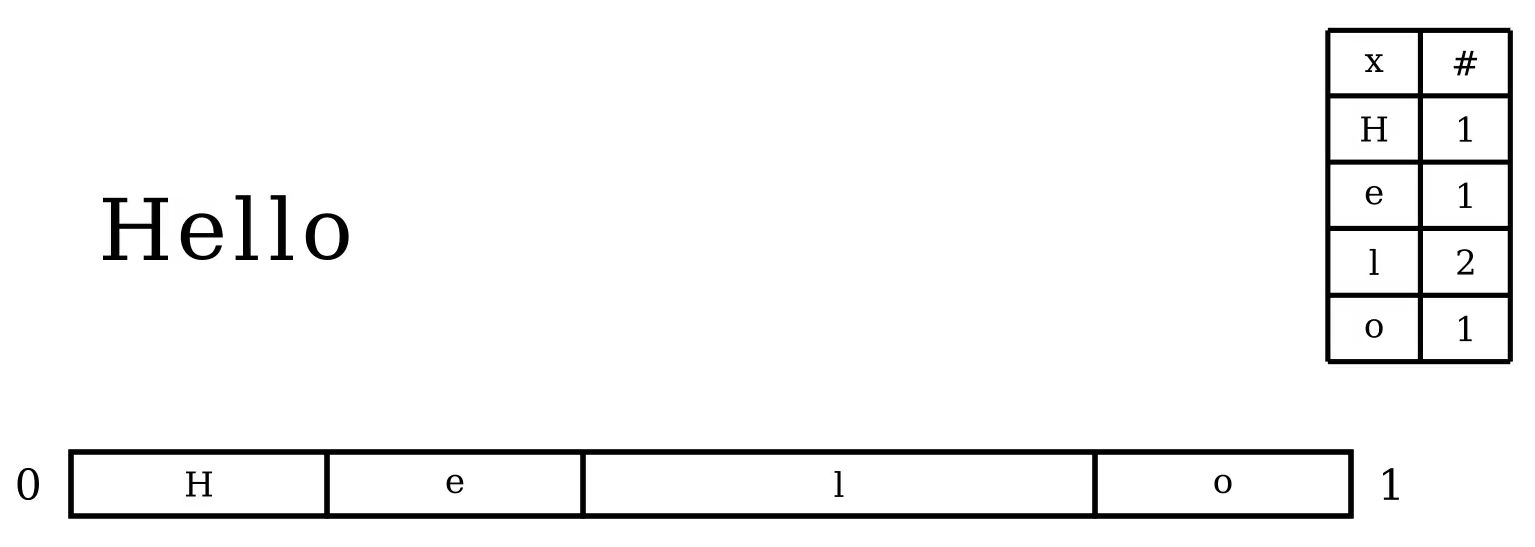
\includegraphics[scale=0.4]{enc-schritt1}
\end{center}
\newpage
Nun wird das erste Zeichen eingelesen. Dessen Intervall wird nun das komplette Intervall ersetzen. Die Verhältnisse der Intervalle untereinander ändert sich nicht. Es werden lediglich die Grenzen aktualisiert. Anschließend wird das nächste Zeichen eingelesen und die Intervallgrenzen entsprechend aktualisiert. Hat man dies nun für alle Zeichen der Eingabe durchgeführt, so liegt einem ein Intervall [a,b] vor.
\begin{center}
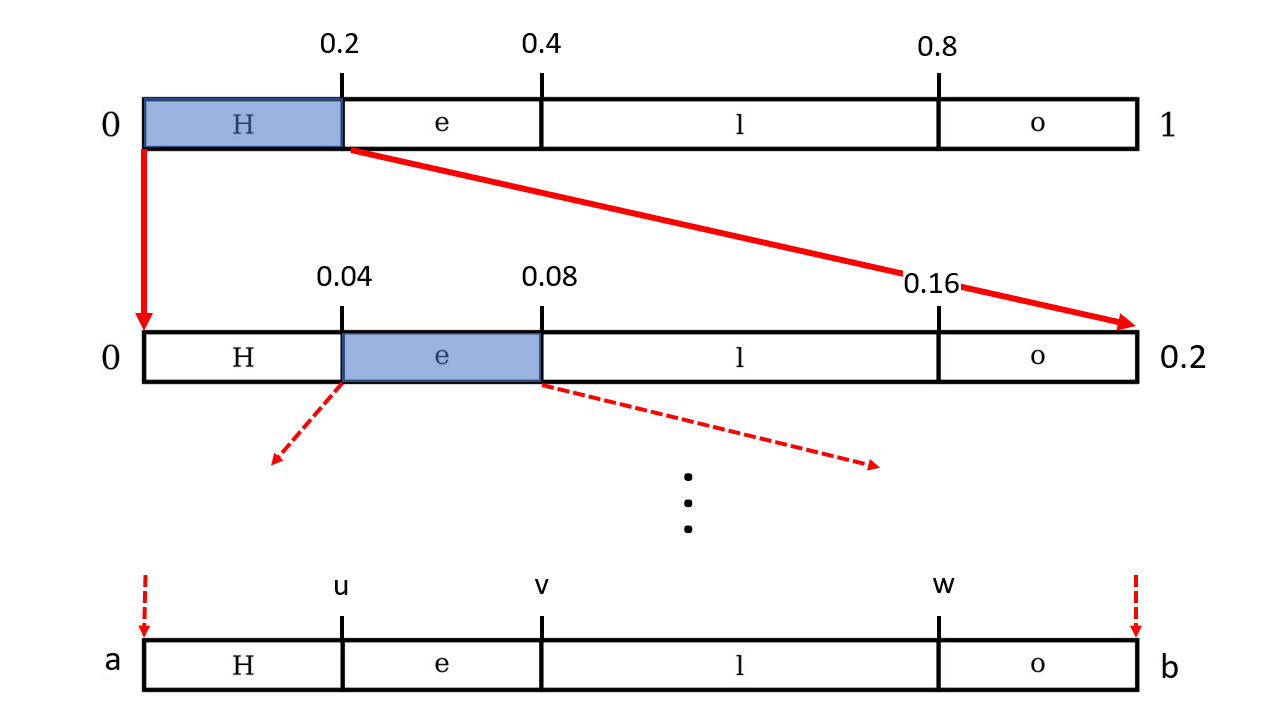
\includegraphics[scale=0.5]{enc-schritt2}
\end{center}
Alle Zahlen innerhalb dieses Intervalls sind korrekte Kodierungen für unsere Eingabe. Es gibt somit theoretisch unendlich viele Kodierungen für eine Eingabe x, nämlich alle Zahlen im Intervall [a,b].\\
Da man bei einer Kodierung eine Eingabe aber natürlich mit möglichst wenig Bits kodieren möchte, wird die kürzeste Binärzahl genommen, welche im Intervall [a,b] liegt.\\
Dies kann z.B. durch einen Binary-Search Algorithmus erreicht werden. So wäre 0.11001 eine mögliche Kodierung für das Interval [0.78, 0.8].

\subsection{Problematik - Finite-Precision Arithmetic Coding}
\label{sec:Problematik}
Normalerweise werden Zahlen mit 32 oder 64 Bit precision gespeichert. Das wird für uns ein Problem, da die Intervallgrenzen sich immer stärker annähern. Dies führt unvermeidlich zu einem Intervall, in welchem beide Grenzen den gleichen Wert annehmen [a,a] und  fortan falsch Kodieren würde.\\
Es existieren mehrere Möglichkeiten, um diese Problematik mehr oder weniger effektiv zu umgehen.\\
Oft wird direkt nach einem kodierten Zeichen geschaut, ob die Zahl im Intervall [0, 0.5] oder [0.5, 1] liegt und das jeweilige Intervall anschließend normalisiert, sodass Rechnungen mit hoher Präzision nie auftreten.

\newpage
\subsection{Dekodierung}
Hier wird als Eingabe ein kodierte Binärzahl x erwartet. Diese wird anschließend in eine Dezimalzahl umgerechnet. Ebenso wird eine Häufigkeitsverteilung aller Zeichen als Eingabe erwartet. Aus dieser wird analog zu \ref{sec:Verfahren-Kodierung} das Intervall [0,1] im Hinblick auf die Zeichen aufgeteilt. Eine Startbedingung könnte folgendermaßen aussehen:
\begin{center}
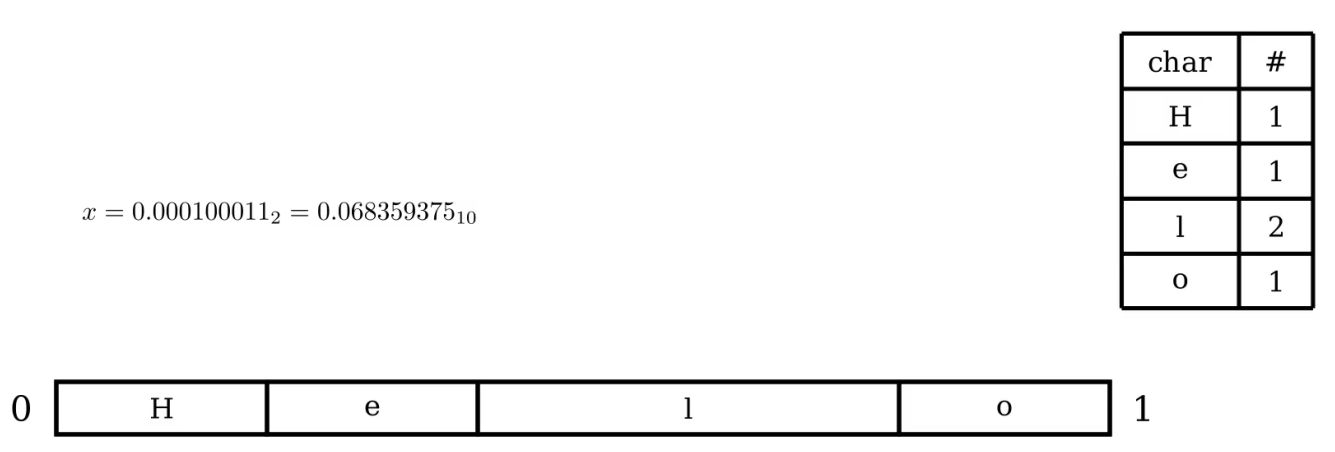
\includegraphics[scale=0.5]{dec-schritt1}
\end{center}
Durch die Häufigkeitsangaben wissen wir, dass die Dekodierung aus genau 5 Zeichen besteht.\\
Im ersten Schritt wird die Dezimalzahl x auf dem Intervall gesucht. Das kodierte Zeichen entspricht nun dem Intervall in welchem sich x befindet \textit{(also H)}.
\\
Anschließend werden die Intervallgrenzen analog zu \ref{sec:Verfahren-Kodierung}
aktualisiert und x erneut auf dem Intervall [0, 0.2] gesucht.
\begin{center}
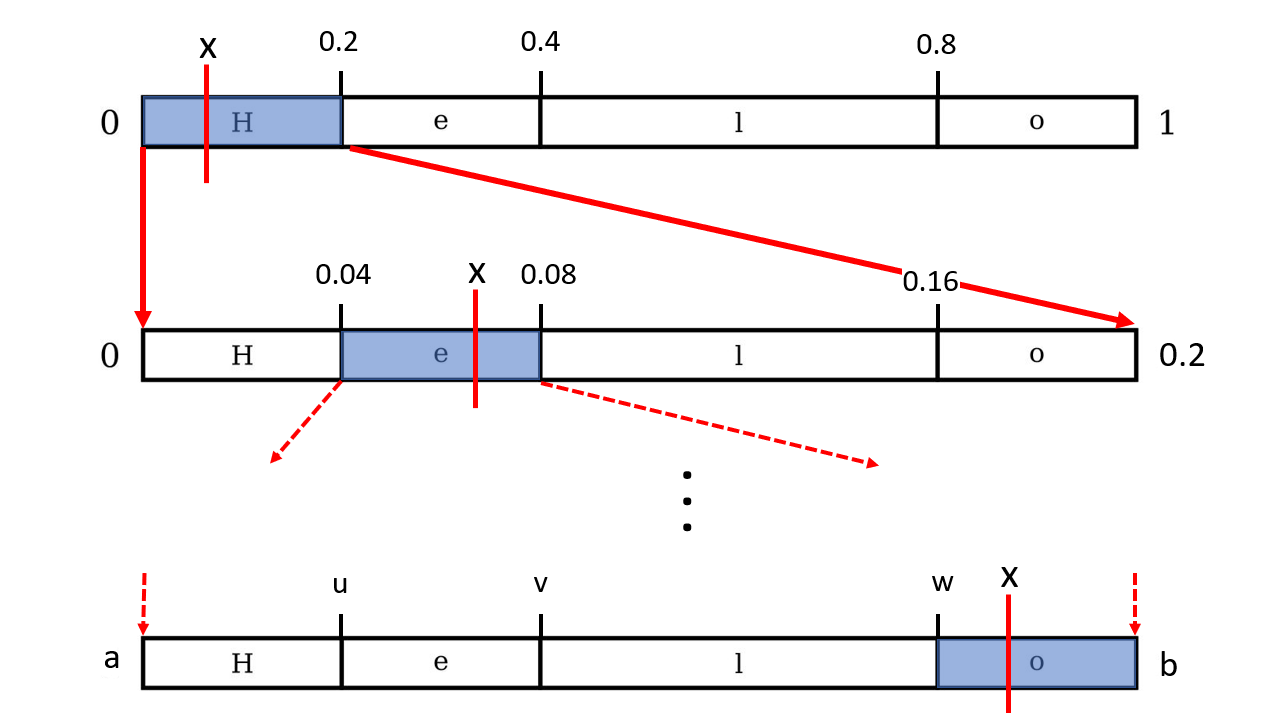
\includegraphics[scale=0.5]{dec-schritt2}
\end{center}
Haben wir dies 5 mal durchgeführt erhalten wird unseren dekodierten String \textit{(Hello)}.
\newpage

		\section{Anwendungsgebiet}
	Implementierungen der Arithmetischen Kodierung können in der Text und Bildkompression genutzt werden. In Bildkompressionsoftware wird nur  teilweise die Arithmetischen Kodierung als Entropie Kodierung genutzt. Aufgrund einer unklaren Patent Situation um die 1980er Jahre, wurde die Huffman-Kodierung oft bevorzugt\cite{WIKI-EN}. JPEG zum Beispiel bietet jedoch beide Entropie-Kodierungen an, wobei eine Konvertierung von Huffman- zu Arithmetischer-Kodierung eine weitere Reduktion von bis zu 25\% erreichen kann.
	
			\section{Qualitätsbewertung über das Verfahren}
	Die Arithmetische Kodierung kommt mit einer genauen Wahrscheinlichkeitstabelle des genutzten Alphabets nahe an das theoretische Limit der Datenkompression: der Entropie der Nachricht. Dabei kann es bessere Ergebnisse als die Huffman-Codierung erreichen, weist dafür jedoch auch einen höheren Rechenaufwand auf, da der Algorithmus komplizierter ist.\\
	Die Asymmetric Numeral Systems (ANS)\cite{WIKI-ANS} kombinieren die nahe an der Entropie liegende Kompressionsrate dieses Verfahrens mit einer, der Huffman-Codierung vergleichbaren, Ausführungszeit.\\
	Die Arithmetische Kodierung liefert also sehr gute Ergebnisse, aber benötigt dafür auch viele Rechenoperationen. Texte mit Millionen Zeichen können in Bruchteilen einer Sekunde komprimiert werden, aber wenn man große Mengen Bilder komprimieren will, kann man noch etwas mehr (zeitliche) Effizienz mit anderen Verfahren herausholen.
	
	\newpage
			\section{Präsentation / Demonstration Kit}
Wir haben bei der Visualisierung/der Umsetzung des Demonstrations Kit zwischen 2 Fällen unterschieden. Da es bei den Berechnungen während der Kodierung/Dekodierung zu Schwierigkeiten mit den Intervallgrenzen kommt (siehe \ref{sec:Problematik}), haben wir ein \textbf{naives} und ein \textbf{genaues} Kit erstellt.
\\
\\
Das naive Kit erstellt eine gut verständliche, visuelle Animation. Jedoch funktioniert dieses Verfahren nur für relativ kleine Eingaben wie z.B ``Hello'' oder ``Laterne''. Bei größeren Eingaben benötigt die Erstellung der Animation erheblich länger. Da dieses Verfahren auch nicht das \textit{Finite-Precision Arithmetic Coding} umsetzt, kommt es hier bei größeren Eingaben zu den in \ref{sec:Problematik} erwähnten Fehlern. Auf kurzen Eingaben ist jedoch eine korrekte
Kodierung/Dekodierung, sowie eine Erstellung einer visuell ansprechenden Animation kein Problem. 
\\
\\
Hierfür haben wir auf das python-Modul \textbf{manim} zurückgegriffen. Dabei handelt es sich um ein Opensource-Projekt des Youtubers ``3Blue1Brown'', welcher es 2015 geschrieben hat, um visuell ansprechende Animationen für den Bereich der Mathematik zu erstellen.\cite{3blue1brown}
\\
Mittlerweile wird dieses Model jedoch durch die Community erweitert und bietet viele Möglichkeiten Themen aus dem MINT-Bereich visuell darzustellen.
\subsection{naives Verfahren}
\label{sec:manim}
\subsubsection{Installation}
Es wird das python-modul \textbf{manim}, sowie viele kleine weitere module wie z.B. \textbf{ffmpeg} benötigt, welche jedoch automatisch mit \textbf{manim} heruntergeladen werden.\\
Der Installationsvorgang wird unter \href{https://docs.manim.community/en/stable/installation.html}{https://docs.manim.community/en/stable/installation.html}
genauer beschrieben.
\\
\subsubsection{Kodierung}
Für die Kodierung wird die Datei \textbf{encoding.py} mithilfe des Befehls
\begin{lstlisting}[language=bash,
numbers=none]
manim -pql -v critical encoding.py
\end{lstlisting}
im terminal ausgeführt.
\\
Anschließend wird als Eingabe das zu kodierende Wort erfragt. Hier wie oben erwähnt, kein zu langes Wort eingeben.
Daraufhin kann es je nach länge des Wortes 1-2 min dauern, bis die Animation erstellt
wurde, welche sich direkt in einem neuen Fenster öffnet und angeschaut werden kann.
Alternativ wurde die Animation unter
\begin{lstlisting}[language=bash, numbers=none]
.\SeminarDatenkompression-2022\pythno\media\videos%encodin\480p15\Encoding.mp4
\end{lstlisting}
gespeichert.
\newpage
\subsubsection{Dekodierung}
Für die Dekodierung wird die Datei \textbf{decoding.py} mithilfe des Befehls
\begin{lstlisting}[language=bash,
numbers=none]
manim -pql -v critical decoding.py
\end{lstlisting}
im terminal ausgeführt.
Anschließend wird als Eingabe zuerst die zu dekodierende Binärzahl
erfragt. Daraufhin wird eine Häufigkeitsverteilung der vorkommenden Buchstaben erfragt.
Diese muss im Format eines python-Dictionaries eingegeben werden.
\\
Beispiele:
\begin{lstlisting}[language=bash,
numbers=none]
{"H": 1, "e": 1, "l": 2, "o": 1}
{"A": 1, "e": 1, "f": 2}
\end{lstlisting}
Daraufhin kann es je nach Länge des Wortes mehrere Minuten dauern, bis die Animation erstellt wurde, welche sich direkt in einem neuen Fenster öffnet und angeschaut werden kann.
Alternativ wurde die Animation unter
\begin{lstlisting}[language=bash,
numbers=none]
.\Seminar-Datenkompression-2022\python%\media\videos\decodin\480p15\Decoding.mp4
\end{lstlisting}
gespeichert.

\subsection{genaues Verfahren}
\label{sec:genaues-Verfahren}
Hierfür bitte die html Datei \textbf{Datenkompression.html} unter \textit{./Seminar-Datenkompression-2022/HTML} öffnen. Die erscheinende Seite, implementiert unsere Kodierungen/Dekodierungen gebündelt in einer html. Hier werden jedoch keine Animationen angezeigt. (Verweis auf \ref{sec:manim})
\subsubsection{Kodierung}
Für die Kodierung wird eine Eingabe im Eingabefeld erwartet. Falls gewünscht kann man sich mit dem Button \textbf{Generiere Wahrscheinlichkeiten}, die Wahrscheinlichkeitsverteilung der Eingabe anzeigen lassen.
\\
Um nun eine genaue Kodierung berechnen zu lassen, nach Eingabe ins obere Feld, den Button \textbf{Starte Genaues-Kompressionsverfahren} drücken.
\\
Anschließend wird der kodierte Binärstring im unteren Feld angezeigt.\\

\subsubsection{Dekodierung}
Um den kodierten Binärstring zu dekodieren, sollte man am besten kurz das obere Eingabefeld manuell leeren. Fügt man nun den kodierten Binärstring ins untere Feld ein und drückt auf \textbf{Starte Genaues-Dekompressionsverfahren}, so wird einem die Dekodierung im oberen Feld angezeigt.


\subsection{naive HTML-Kodierung}
Auf der HTML Seite kann man zusätzlich noch einmal das naive Verfahren ausführen lassen. Das Vorgehen ist analog zu \ref{sec:genaues-Verfahren}.\\
\textit{Anmerkung: Die Kodierung weicht leicht von der Kodierung in den Animationen ab, da der Algorithmus anders implementiert wurde.}


	
	
	
% wird am Ende entfernt. Dient nur zur Referenz für gewisse commands

		
		\newpage
	
	\begin{thebibliography}{2}
		\bibitem{mark-nelson} Mark Nelson. (2014, October 19). Data compression with arithmetic coding. Mark Nelson. Retrieved January 12, 2023, from https://marknelson.us/posts/2014/10/19/data-compression-with-arithmetic-coding.html 

\bibitem{go} Arithmetic coding. The Hitchhiker's Guide to Compression. (n.d.). Retrieved January 15, 2023, from https://go-compression.github.io/algorithms/arithmetic/ 
		
		\bibitem{WIKI} Wikimedia Foundation. (2022, November 6). Arithmetisches Kodieren. Wikipedia. Retrieved January 12, 2023, from https://de.wikipedia.org/wiki/Arithmetisches\_Kodieren
		
		\bibitem{WIKI-EN} Wikimedia Foundation. (2023, January 21). Arithmetic coding. Wikipedia. Retrieved January 23, 2023, from https://en.wikipedia.org/wiki/Arithmetic\_coding
	
		\bibitem{3blue1brown} Wikimedia Foundation. (2022, December 30). 3Blue1Brown. Wikipedia. Retrieved January 15, 2023, from https://en.wikipedia.org/wiki/3Blue1Brown 
	
		\bibitem{WIKI-ANS} Wikimedia Foundation. (2022, August 9). Asymmetric Numeral Systems. Wikipedia. Retrieved January 23, 2023, from https://de.wikipedia.org/wiki/Asymmetric\_Numeral\_Systems	
			\end{thebibliography}
\end{document}